%---------- Inleiding ---------------------------------------------------------

\section{Introductie} % The \section*{} command stops section numbering
\label{sec:introductie}

% Hier introduceer je werk. Je hoeft hier nog niet te technisch te gaan.

% Je beschrijft zeker:

% \begin{itemize}
%   \item de probleemstelling en context
%   \item de motivatie en relevantie voor het onderzoek
%   \item de doelstelling en onderzoeksvraag/-vragen
% \end{itemize}


Voor cloud-providers is het belangrijk om in te schatten wat de performantie impact zal zijn voor de Meltdown/Spectre patches.
Een vergelijkende studie met genoeg scenario's is aan de orde. Een scenario kan bijvoorbeeld bandbreedte zijn.
Dit onderzoek moet duidelijke resultaten geven over het verlies van performantie. Ook moet deze bachelorproef uitleg geven over de risicobeperkende maatregelen en waarom ze slechte performantie geven.

%---------- Stand van zaken ---------------------------------------------------

\section{State-of-the-art}
\label{sec:state-of-the-art}

% Hier beschrijf je de \emph{state-of-the-art} rondom je gekozen onderzoeksdomein. Dit kan bijvoorbeeld een literatuurstudie zijn. Je mag de titel van deze sectie ook aanpassen (literatuurstudie, stand van zaken, enz.). Zijn er al gelijkaardige onderzoeken gevoerd? Wat concluderen ze? Wat is het verschil met jouw onderzoek? Wat is de relevantie met jouw onderzoek?

% Verwijs bij elke introductie van een term of bewering over het domein naar de vakliteratuur, bijvoorbeeld~\autocite{Doll1954}! Denk zeker goed na welke werken je refereert en waarom.

% Voor literatuurverwijzingen zijn er twee belangrijke commando's:
% \autocite{KEY} => (Auteur, jaartal) Gebruik dit als de naam van de auteur
%   geen onderdeel is van de zin.
% \textcite{KEY} => Auteur (jaartal)  Gebruik dit als de auteursnaam wel een
%   functie heeft in de zin (bv. ``Uit onderzoek door Doll & Hill (1954) bleek
%   ...'')

% Je mag gerust gebruik maken van subsecties in dit onderdeel.

Sinds dit een nieuw probleem is, zijn er nog niet veel academische onderzoeken.
Redhat zegt wel dat Meltdown en Spectre een impact van 0 tot 19 percent heeft \autocite{Redhat2018}.
%---------- Methodologie ------------------------------------------------------
\section{Methodologie}
\label{sec:methodologie}

% Hier beschrijf je hoe je van plan bent het onderzoek te voeren. Welke onderzoekstechniek ga je toepassen om elk van je onderzoeksvragen te beantwoorden? Gebruik je hiervoor experimenten, vragenlijsten, simulaties? Je beschrijft ook al welke tools je denkt hiervoor te gebruiken of te ontwikkelen.

De testopstelling wordt gemaakt met Vagrant en Ansible. Vagrant wordt gebruikt voor het maken van de virtuele machines en instellingen zoals ip-adressen. Ansible wordt gebruikt voor de configuratie van de software. Het doel is om data op te slaan met een paar benchmark-tools en analyseren met SPSS of R.

%---------- Verwachte resultaten ----------------------------------------------
\section{Verwachte resultaten}
\label{sec:verwachte_resultaten}

% Hier beschrijf je welke resultaten je verwacht. Als je metingen en simulaties uitvoert, kan je hier al mock-ups maken van de grafieken samen met de verwachte conclusies. Benoem zeker al je assen en de stukken van de grafiek die je gaat gebruiken. Dit zorgt ervoor dat je concreet weet hoe je je data gaat moeten structureren.

\begin{figure}
	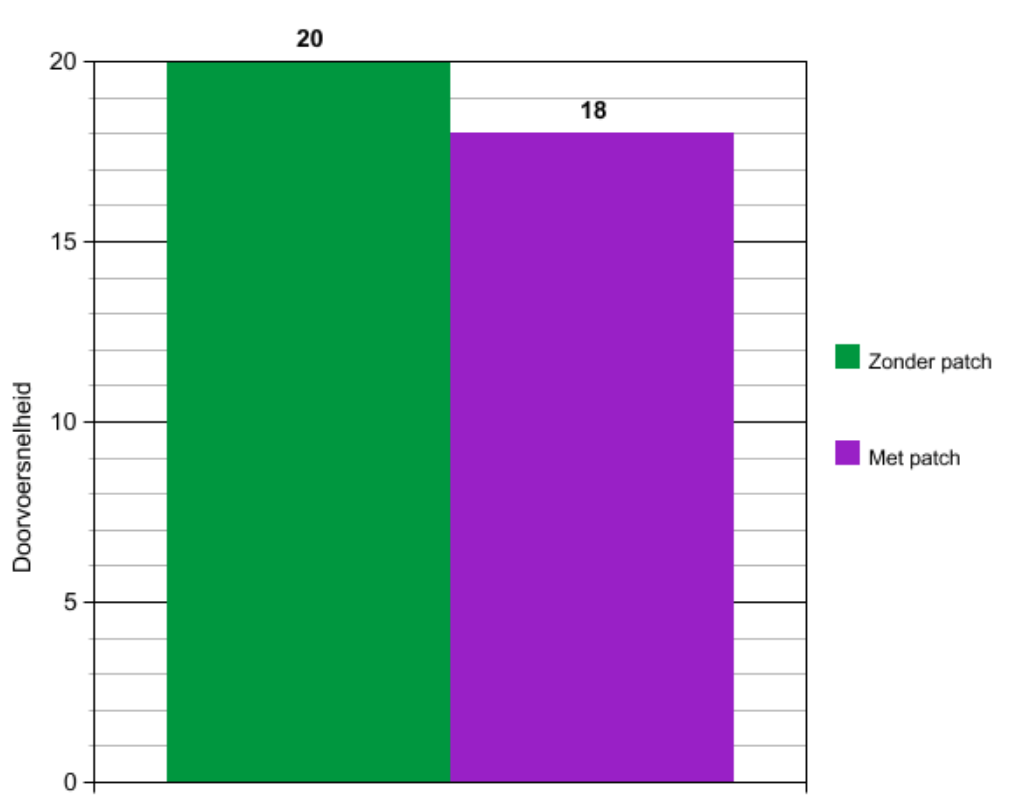
\includegraphics[width=1.0\linewidth]{../voorstel/voorstel.png}
	\caption{Mockup}
	\label{fig:voorstel}
\end{figure}

Figuur \ref{fig:voorstel} is een mock-up van de doorvoersnelheid.



%---------- Verwachte conclusies ----------------------------------------------
\section{Verwachte conclusies}
\label{sec:verwachte_conclusies}

% Hier beschrijf je wat je verwacht uit je onderzoek, met de motivatie waarom. Het is \textbf{niet} erg indien uit je onderzoek andere resultaten en conclusies vloeien dan dat je hier beschrijft: het is dan juist interessant om te onderzoeken waarom jouw hypothesen niet overeenkomen met de resultaten.

Een hoogstwaarschijnlijke conclusie kan zijn dat de patches een significante impact hebben, maar dat ze niet desastreus zijn. Het is ook zeker interessant om op te volgen wat de grote processorfabrikanten en besturingssysteemontwikkelaars gaan doen met betrekking tot updates en nieuwe processorarchitecturen.